\section{Charged leptons in cosmic plasma}\label{Electron}

Charged leptons played significant roles in the dynamics and evolution of the early Universe. They were kept in equilibrium via electromagnetic and weak interactions.  In this chapter, we examine a dynamical model of the abundance of charged leptons $\mu^\pm$ and $e^\pm$ in the early Universe obtaining their disappearance temperature, the condition when they disappear from the particle inventory. Of particular interest is the dense electron-positron plasma present during the early Universe evolution. We study the damping rate and the magnetization process in this dense $e^\pm$ plasma in the early Universe.

%%%%%%%%%%%%%%%%%%%%%%%%%%%%%
\subsection{Timeline for charged leptons in early Universe}

The $\tau^\pm$ leptons can undergo various decay processes via the weak interaction in the early Universe, and is the only charged lepton that can decay into hadrons because of its heavy mass ($m_\tau=1776.86$ MeV). The principle decay channels of $\tau^\pm$ are given by
\begin{align}
&\tau^-\rightarrow\nu_\tau+e^-+\bar{\nu}_e,\qquad \tau^-\rightarrow\nu_\tau+\mu^-+\bar{\nu}_\mu,\\
&\tau^-\rightarrow\nu_\tau+\pi^-,\qquad\qquad\,\tau^+\rightarrow\bar{\nu}_\tau+\pi^+,
\end{align}
 where the vacuum lifespan for $\tau^\pm$ is given by ~\cite{ParticleDataGroup:2022pth}
\begin{align}
&\tau_{\tau}=(290.3\pm0.5)\times10^{-15}\,\mathrm{sec}\,.
\end{align}

Moreover, following the decay of $\tau^\pm$ into pions, these pions subsequently decay into a muon and a neutrino through the reaction
\begin{align}
\pi^-\rightarrow\nu_\mu+\mu^-,\qquad\qquad\,\pi^+\rightarrow\bar{\nu}_\mu+\mu^+,
\end{align}
with pion vacuum lifespan $\tau_\pi=2.6033\times10^{-8}$ sec~\cite{ParticleDataGroup:2022pth}.
In this scenario, $\tau^\pm$ disappears from the Universe via multiparticle decay processes.
These decay processes can contribute as one of the sources for the production of neutrinos and muons in the early Universe.

The $\mu^\pm$ lepton abundance is an important quantity required for the understanding of several fundamental questions regarding properties of the primordial Universe,  particularly in relation to the freeze-out of strangeness flavor in the early Universe. We recall that the strangeness decay often proceeds into muons, energy thresholds permitting, as the charged kaons K$^\pm$ have a 63\% branching into $\mu+\bar \nu_\mu$. Should muons fall out of thermal abundance equilibrium this would directly impact the detailed balance back-reaction processes. Another, indirect influence on strangeness in early Universe arises through the nearly exclusive decay of charged pions into $\mu+\bar \nu_\mu$. Without chemical abundance equilibrium this back reaction stops too impacting pions and thus all other hadronic particles in the Universe. 

On the other hand, we will show that the lightest charged leptons $e^\pm$ can persist via the reaction $\gamma\gamma\to e^-e^+$ until the temperature $T=20$ keV in the early Universe.  After $T=20$ keV, the positron rapidly disappears through annihilation, leaving only residual electrons to maintain the Universe's charge neutrality. The existence of an electron-positron plasma plays a pivotal role in several aspects of the early Universe as follows: 

1. The role of electron-positron plasma has not received the appropriate attention in the days of precision Big-Bang nucleosynthesis studies. The standard BBN model indicates that the synthesis of light elements typically takes place at temperatures around  $86\,\mathrm{keV}>T_{BBN}>50\,\mathrm{keV}$~\cite{Pitrou:2018cgg}. Within this temperature range there are millions of electron-positron pairs per charged nucleon, providing an electron-positron-rich plasma environment for nucleosynthesis which leads to modifications in the Coulomb potential due to the screening effect. Furthermore, the electron-positron densities can reach millions of times normal atomic densities. The presence of  these $e\bar e$-pairs before and during BBN has been acknowledged by Wang, Bertulani and Balantekin~\cite{Wang:2010px} nearly a decade ago.

2. The Universe today is filled with magnetic fields at various scales and strengths both within galaxies and in deep extra-galactic space. The origin of these magnetic fields is currently unknown. In the early Universe, when temperature $T>20$ keV, we have dense $e^\pm$ plasma. The significant magnetic moments of electrons and positrons also provide opportunities to investigate spin magnetization process.

Understanding the abundances of muons and electrons/positrons provides essential insights into the evolution of the primordial Universe.  In the following we discuss the muon density at persistence temperature in section \ref{section_muon}, and explore the electron/positron plasma properties, including the damped rate and magnetization in section \ref{section_electron}.

%%%%%%%%%%%%%%%%%%%%%%%%%%%%%%%%%%%%%%%
\paragraph{Muon–antimuon in the early Universe}\label{section_muon}

Our interest in strangeness flavor freeze-out in the early Universe requires the understanding of the abundance of muons in the early Universe. The specific question needing an answer is at which temperature muons remain in abundance (chemical) equilibrium established predominantly by electromagnetic and weak interaction processes, allowing detailed-balance back-reactions to influence strangeness abundance.

In the early Universe in the the cosmic plasma muons of mass $m_\mu=105.66$\,MeV can be produced by the following interaction processes
\begin{align} 
&\gamma+\gamma\longrightarrow\mu^++\mu^-,\qquad & e^++e^-\longrightarrow \mu^++\mu^-\;,\\
&\pi^-\longrightarrow\mu^-+\bar{\nu}_\mu,\qquad & \pi^+\longrightarrow\mu^++\nu_\mu\;.
\end{align}
The back reactions for all above processes are in detailed balance, provided all particles shown on the right hand side (RHS) exist in chemical abundance equilibrium in the Universe. We recall the empty space (no plasma) at rest lifetime of pions $\tau_\pi=2.6033\times10^{-8}$ sec. 

However, all produced muons can also decay via the reactions
\begin{equation}
\mu^-\rightarrow\nu_\mu+e^-+\bar{\nu}_e,\qquad \mu^+\rightarrow\bar{\nu}_\mu+e^++\nu_e\,,
\end{equation} 
with the empty space (no plasma) at rest lifetime $\tau_{\mu}=2.197 \times 10^{-6}\,\mathrm{sec}$. We thus must establish the range of temperature in which production processes exceed in speed the decay process.
 
The temperature range of our interests is the Universe when $m_\mu\gg T$. In this case the the Boltzmann approximation is appropriate for studying massive particles muons and pions. The thermal decay rate per volume and time  for muons $\mu^\pm$ (and pions $\pi^\pm$) in the Boltzmann limit  are given by~\cite{PhysRevC.82.035203}:\index{muon decay rate}
\begin{align}
&R_\mu=\frac{g_\mu}{2\pi^2}\left(\frac{T^3}{\tau_\mu}\right)\left(\frac{m_\mu}{T}\right)^2K_1(m_\mu/T)\;,\\
&R_\pi=\frac{g_\pi}{2\pi^2}\left(\frac{T^3}{\tau_\pi}\right)\left(\frac{m_\pi}{T}\right)^2K_1(m_\pi/T)\;, 
\end{align}
where the lifespan of $\mu^\pm$ and $\pi^\pm$ in the vacuum were given above. This rate accounts for both the density of particles in chemical abundance equilibrium and the effect of time dilation present when particles are in thermal motion with respect to observer at rest in the local reference frame. The effects of Fermi blocking or boson stimulated emission have been neglected.

The thermal averaged reaction rate per volume for the reaction $a\overline{a}\rightarrow b\overline{b}$ in Boltzmann approximation is given by \cite{Letessier:2002ony}\index{muon prodution rate}
\begin{align}\label{pairR}
R_{a\overline{a}\rightarrow b\overline{b}}=\frac{g_ag_{\overline{a}}}{1+I}\frac{T}{32\pi^4}\int_{s_{th}}^\infty ds\frac{s(s-4m^2_a)}{\sqrt{s}}\sigma_{a\overline{a}\rightarrow b\overline{b}}~K_1(\sqrt{s}/T),
\end{align}
where $s_{th}$ is the threshold energy for the reaction, $\sigma_{a\overline{a}\rightarrow b\overline{b}}$ is the cross section for the given reaction, and $K_1$ is the modified
Bessel function of integer order ``$1$". We introduce the factor $1/1+I$ to avoid the double counting of indistinguishable pairs of particles; we have $I=1$ for an identical pair and $I=0$ for a distinguishable pair.

The leading order invariant matrix elements for the reactions $e^++e^-\to\mu^++\mu^-$ and $\gamma+\gamma\to\mu^++\mu^-$, are introduced in this work by \cite{Kuznetsova:2008jt}
\begin{align}\label{Mee}
|M_{e\bar e\to\mu\bar\mu}|^2=&32\pi^2\alpha^2\frac{(m_\mu^2-t)^2+(m_\mu^2-u)^2+2m_\mu^2s}{s^2},\quad m_\mu\gg m_e\;,\\[0.2cm]
\label{Mgg}
|M_{\gamma\gamma\to\mu\bar\mu}|^2=&32\pi^2\alpha^2\bigg[\left(\frac{m_\mu^2-u}{m_\mu^2-t}+\frac{m_\mu^2-t}{m_\mu^2-u}\right)+4\left(\frac{m_\mu^2}{m_\mu^2-t}+\frac{m_\mu^2}{m^2_\mu-u}\right)\\[0.1cm]  \nonumber
&\hspace{1cm}-4\left(\frac{m_\mu^2}{m^2_\mu-t}+\frac{m^2_\mu}{m^2_\mu-u}\right)^2\bigg]\;,
\end{align}
 where $s, t, u$ are the Mandelstam variables. The cross section required in Eq.\,(\ref{pairR}) can be obtained by integrating the matrix elements Eq.\,(\ref{Mee}) and Eq.\,(\ref{Mgg}) over the Mandelstam variable $t$ ~\cite{PhysRevC.82.035203}. We have
\begin{align}
&\sigma_{e\bar e\to\mu\bar\mu} 
=\frac{64\pi\alpha^2}{48\pi}\left(\frac{1+2m^2_\mu/s}{s-4m_e^2}\right)\sqrt{1-\frac{4m^2_\mu}{s}},\\
&\sigma_{\gamma\gamma\to\mu\bar\mu}=\frac{\pi}{2}\left(\frac{\alpha}{m_\mu}\right)^2(1-\beta^2)\left[(3-\beta^4)\ln\frac{1+\beta}{1-\beta}-2\beta(2-\beta^2)\right],\\
&\beta=\sqrt{1-4m^2_\mu/s}
\end{align}
Substituting the cross sections into Eq.\,(\ref{pairR}) we obtain the production rates for $e\bar e\to\mu\bar\mu$ and $\gamma\gamma\to\mu\bar\mu$ respectively.

 
In Fig.~\ref{MuonRatenew_fig} we show the invariant thermal reaction rates per volume and time for rates of relevance, as a function of temperature $T$.
As the temperature decreases in the expanding Universe, the initially dominant production rates ($e\bar e,\gamma\gamma\to\mu\bar\mu$) decrease with decreasing temperature, and eventually cross the $\mu^\pm$ decay rates. 
Muon abundance disappears as soon as any decay rate is faster than the fastest production rate. Specifically after the Universe cools below the temperature $T_\mathrm{disappear}=4.195$ MeV, the dominant reaction is the muon decay. Due to the relatively slow expansion of the Universe, the disappearance of muons is sudden, and the abundance of muons vanishes as soon as a decay rate surpasses the dominant production rate.
 
%%%%%%%%%%%%%%%%%%%%%%%%%%
\begin{figure}
\centerline{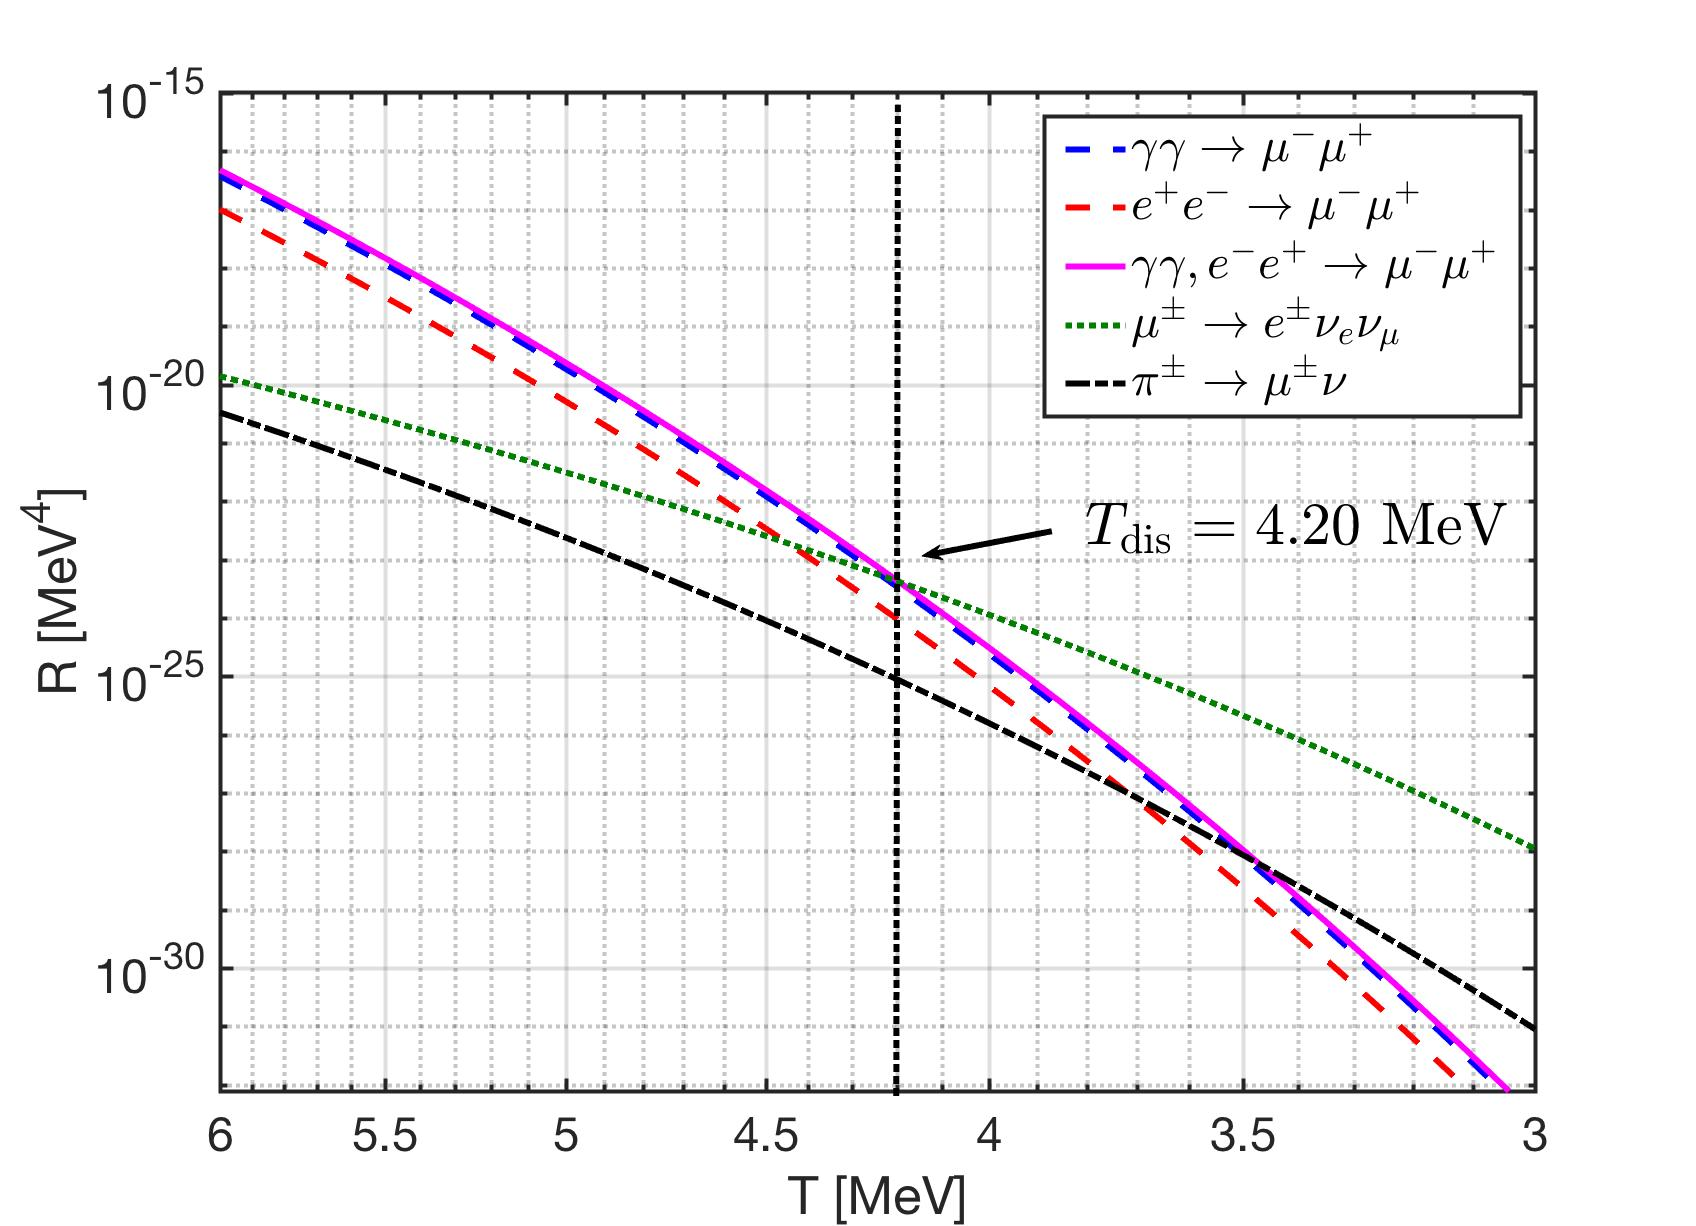
\includegraphics[width=0.9\textwidth]{./plots/MuonRate_new2.jpg}}
\caption{\cccite{Rafelski:2023emw}, adapted from Ref.~\cite{Rafelski:2021aey} and thesis of C.T.Yang \cite{Yang:2024ret}. The thermal reaction rate per unit time and units volume for different reactions as a function of temperature. The dominant reactions for $\mu^\pm$ production are ${\gamma+\gamma\to\mu^++\mu^-}$ and $e^++e^-\to\mu^++\mu^-$, and the total production rate crosses the decay rate of $\mu^\pm$ at temperature $T_{dissapear}\approx 4.195$ MeV}
\label{MuonRatenew_fig} 
\end{figure}
%%%%%%%%%%%%%%%%%%%%%%%%%%%%%%

On the other hand, considering the number density for nonrelativistic $\mu^\pm$ in the Boltzmann approximation, we have
\begin{align}\label{nmupm}
n_{\mu^\pm}=\frac{g_{\mu^\pm}}{2\pi^2}T^3\left(\frac{m_\mu}{T}\right)^2 K_2(m_\mu/T)=g_{\mu^\pm}\left(\frac{m_\mu T}{2\pi}\right)^{3/2}e^{-{m_\mu}/{T}}\;. 
\end{align}
then the number density between $n_{\mu^\pm}$ and baryon $n_B$ can be written as
\begin{align}
\frac{n_{\mu^\pm}}{n_\mathrm{B}}=\frac{n_{\mu^\pm}}{s}\frac{s}{n_\mathrm{B}}=
\frac{n_{\mu^\pm}}{s}\left(\frac{s}{n_\mathrm{B}}\right)_{\!t_0},
\end{align}
where we used that $s/n_\mathrm{B}$ remains constant and $t_0$ represent present day value. The present value is given by $(n_B/s)_{t_0}\approx8.69\times10^{-11}$. The entropy density $s$ can be characterized introducing $g^s_\ast$, the total number of \lq entropic\rq\ degrees of freedom
\begin{align}\label{entrop}
s=\frac{2\pi^2}{45}g^s_\ast T^3\;.
\end{align}
For temperature $10\,\mathrm{MeV} >T>3 $\,MeV, the massless photons, nearly relativistic electron/positrons, and practically massless neutrinos contribute to the degree of freedom $g^s_\ast$.  In this case, the number density between $n_{\mu^\pm}$ and baryon $n_B$ in the temperature interval we consider $10\,\mathrm{MeV} >T>3 $\,MeV is given by
\begin{align}\label{nmuperbF} 
\frac{n_{\mu^\pm}}{n_\mathrm{B}}=\frac{45}{2\pi^2}\frac{g_{\mu^\pm}}{g^s_\ast}\left(\frac{m_\mu}{2\pi T}\right)^{3/2}e^{-{m_\mu}/{T}}\;\left(\frac{s}{n_\mathrm{B}}\right)_{\!t_0}.
\end{align}
 
In \rf{fig:DensityRatio} we show the muon to baryon density ratio Eq.\,(\ref{nmuperbF}) as a function of $T$. We see that the muon abundance $T=10$\,MeV exceeds that of baryons by a factor 500,000 while at muon disappearance temperature $n_{\mu^\pm}/n_\mathrm{B}(T_\mathrm{disappear})\approx0.911$. The number density $n_{\mu^\pm}$ and $n_\mathrm{B}$  abundances are equal at around the temperature $T_\mathrm{equal}\approx4.212\,\mathrm{MeV} >  T_\mathrm{disappear}$.  This means that the muon abundance may still be able to influence baryon evolution because their number density is comparable to the baryon density.% However, we also find that at the temperature $T_\mathrm{equal}\approx4.212$\,MeV the density ratio is unity $n_{\mu^\pm}/n_\mathrm{B}\approx1$.

%%%%%%%%%%%%%%%%%%%%%%%%%%%%%%%%%%%%%
\begin{figure}
\centerline{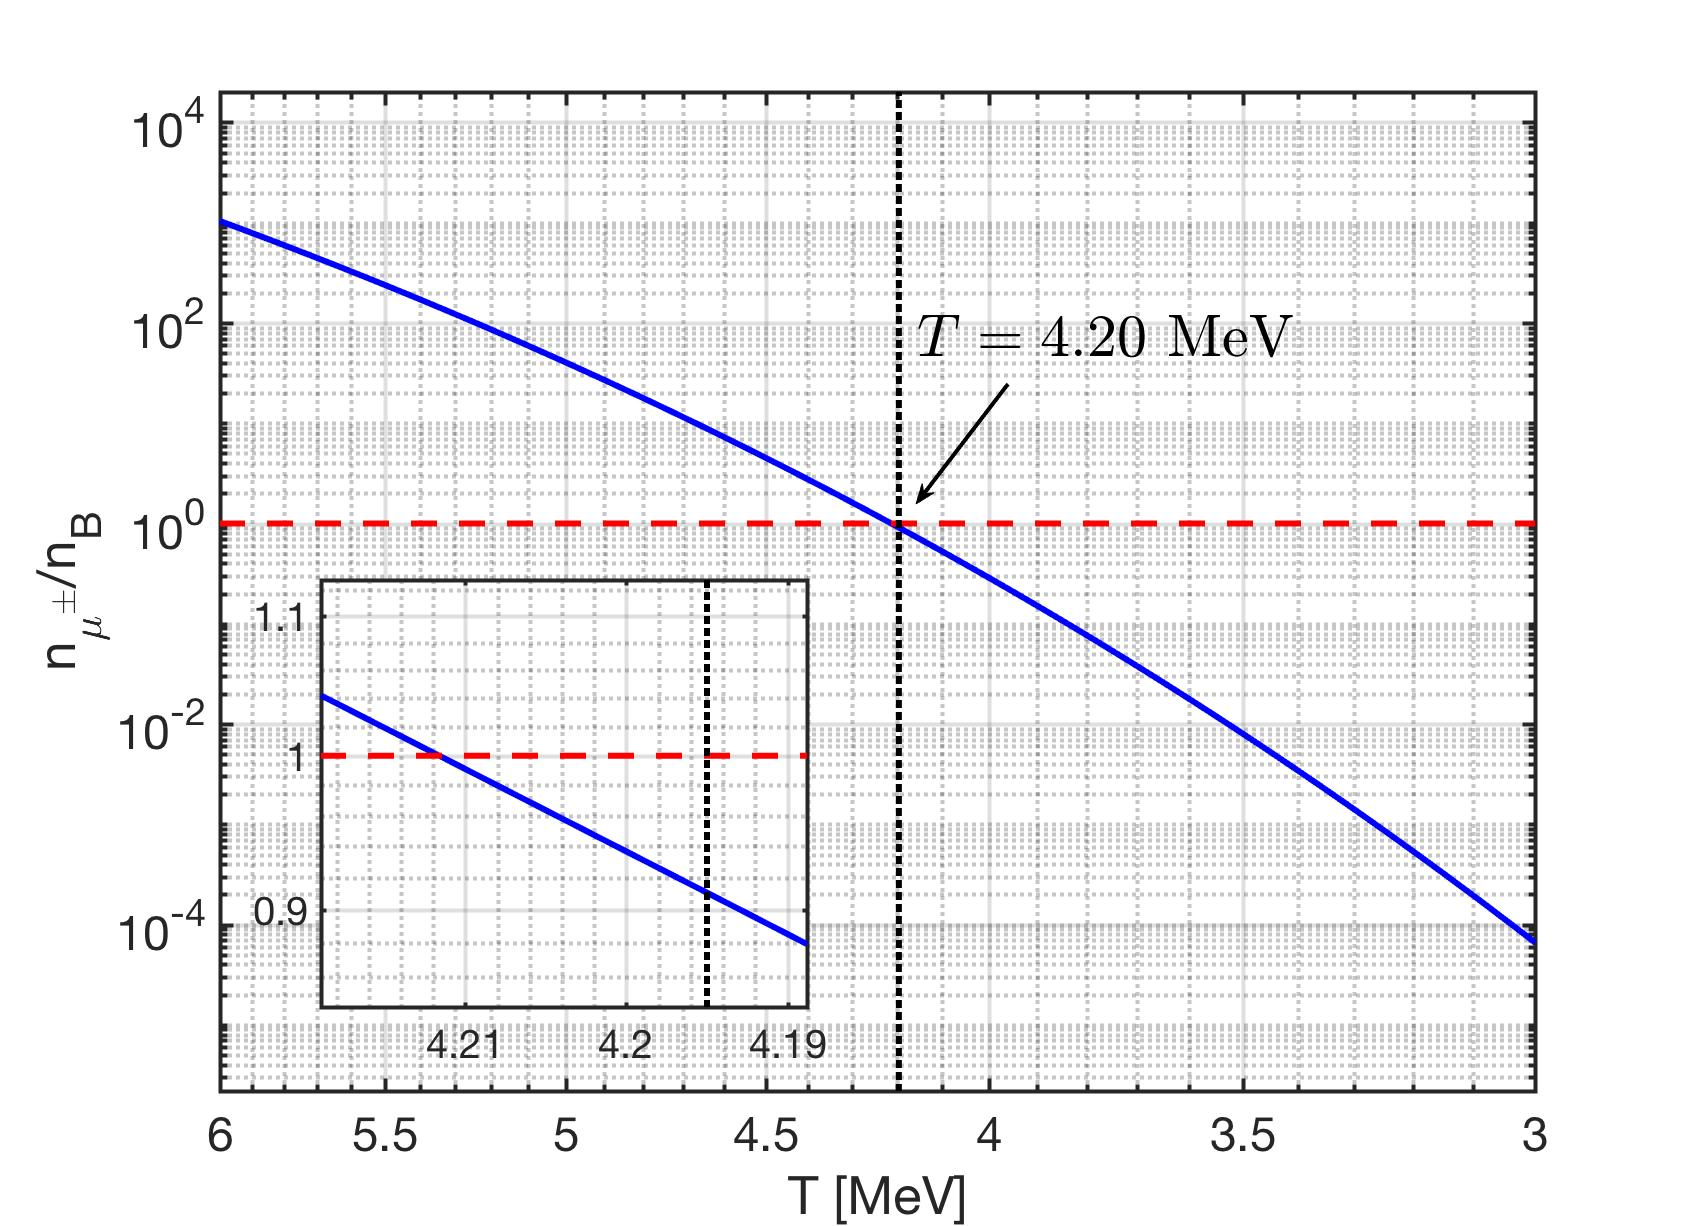
\includegraphics[width=0.9\textwidth]{./plots/DensityRatio_new2.jpg}}
\caption{\cccite{Rafelski:2023emw}, adapted from Ref.~\cite{Rafelski:2021aey} and thesis of C.T.Yang \cite{Yang:2024ret}.
The density ratio between $\mu^\pm$ and baryons as a function of temperature. The density ratio at muon disappearance temperature is about $n_{\mu^\pm}/n_\mathrm{B}(T_\mathrm{disappear})\approx0.911$, and around the temperature $T\approx4.212$ MeV the density ratio $n_{\mu^\pm}/n_\mathrm{B}\approx1$}
\label{fig:DensityRatio}
\end{figure}
%%%%%%%%%%%%%%%%%%%%%%%%

The primary insight of this work is that aside of protons, neutrons and other nonrelativistic particles, both positively and negatively charged muons $\mu^\pm$ are present in thermal equilibrium and in non-negligible abundance for $T>T_\mathrm{dissapear}\approx 4.195$\,MeV. This offers a new and tantalizing model building opportunity for anyone interested in baryon-antibaryon separation in the primordial Universe, strangelet formation, and perhaps other exotic primordial structure formation mechanisms.

%%%%%%%%%%%%%%%%%%%%%%%%%%%%%%%





%%%%%%%%%%%%%%%%%%%%%%%%%%%%%%%%%%%%%%%%%%%%%%%
\subsection{Electron-positron plasma and BBN}
\label{sec:density}

We derive the electron-positron density and chemical potential to show that during the normal BBN temperature range $86.7\,\mathrm{keV}>\mathrm{T_{BBN}}>50\,\mathrm{keV}$~\cite{Pitrou:2018cgg} the Universe was filled with a dense electron-positron pair-plasma dotted with dispersed baryonic matter dust.  Before BBN, for temperatures $T>86.7\,$keV were high enough that any nuclei formed to be disassociated by the vast number of high energy photons present \cite{Pitrou:2018cgg}. 

Once the temperature cooled to around $T<50\,$keV most of the nuclear reactions forming nuclei had already occurred. In this study, we can neglect the universe's expansion since, at this period, the time scale of expansion $H^{-1}$ is orders of magnitude larger than the time scale of BBN. We also note that at this point neutrinos have become free streaming \cite{Birrell:2012gg}.

In Ref.\,\cite{Grayson:2022asf} we used the present-day baryon-to-photon ratio: $B/N_\gamma =n_B/n_\gamma= 6.05\times10^{-10}$ from Cosmic Microwave Background (CMB)~\cite{ParticleDataGroup:2022pth} and the charge neutrality of the universe to find the electron-positron chemical potential and density during BBN.
%%%%%%%%%%%%%%%%%%%%%%%%%%%%%%%%%%%%%%%%%
\begin{figure}  
%\includegraphics[width=0.95\linewidth]{Chemical_Plasma}
%\includegraphics[width=0.95\linewidth]{Density_Plasma002}
\centerline{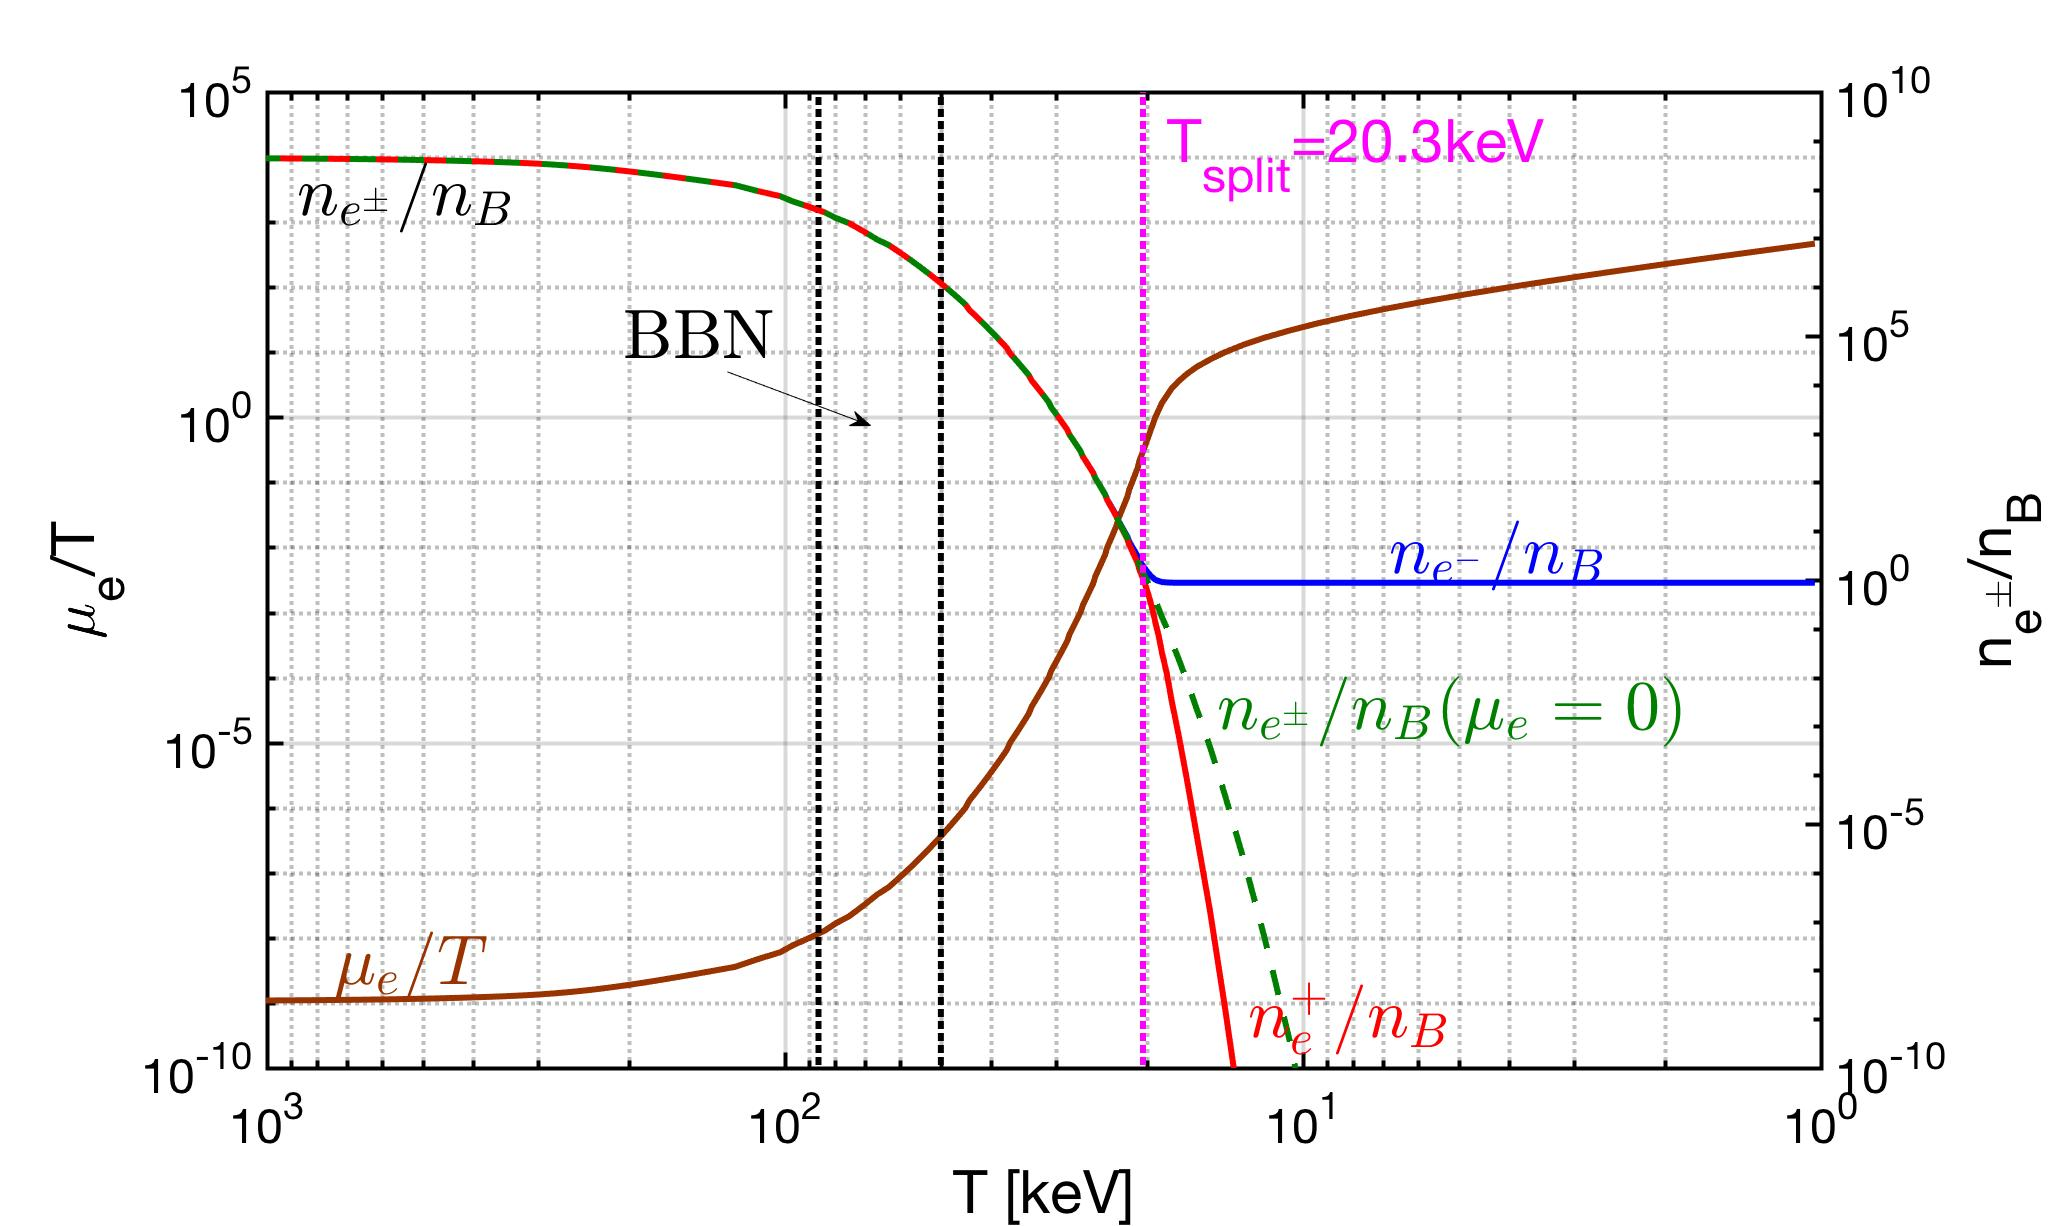
\includegraphics[width=0.90\linewidth]{plots/chap03BBN/May152023_EPDensity_Chemical}}
\caption{\cccite{Grayson:2023flr}, adapted from Ref.~\cite{Grayson:2023flr} and thesis of C.T.\,Yang~\cite{Yang:2024ret}. Left axis: The chemical potential of electrons as a function of temperature. Right axis: the ratio of electron (positron) number density to baryon density as a function of temperature. The solid blue line is the electron density, the red dashed line is the positron density, and the green dotted line is the number density with $\mu_e=0$. When $T=20.3\,\mathrm{keV}$ (the purple vertical line) positron density decreases rapidly because of the annihilation. The vertical black dotted lines represent BBN temperature range $86\,\mathrm{keV}>\mathrm{T_{BBN}}>50\,\mathrm{keV}$}
\label{BBN_Electron} 
\end{figure}
%%%%%%%%%%%%%%%%%%%%%%%%%%%%%%%%%%%%%%%%%%%%%%%%%%%%%

In \rf{BBN_Electron} (left axis), we plot the electron chemical potential as a function of temperature. We can see the value of chemical potential is comparatively small $\mu_e/T\approx10^{-6}\sim10^{-7}$ during the BBN temperature range, implying an equal number of electrons and positrons in plasma. Thus, for the proceeding calculations, we will set $\mu =0$. When the temperature is around $T=70\,\mathrm{keV}$, the density of electrons and positrons is comparatively large $n_{e^\pm}\approx10^7\,n_B$. This indicates that we can assume the universe is filled mainly with electrons and positrons with light nuclei being a very small component of the plasma. Later when the temperature is around $T=20.3\,\mathrm{keV}$, the positron density decreases, transforming the pair-plasma to an electron-baryon plasma.


We next obtain the dependence of electron chemical potential, and hence $e^+e^-$ density, as a function of the photon background temperature $T$ by employing the following physical principles:
\begin{enumerate}
\item Charge neutrality of the Universe:
\begin{align}\label{neutrality}
n_{e^-}-n_{{e^+}}=n_p-n_{\overline{p}}\approx\,n_p,
\end{align}
where $n_\ell$ denotes the number density of particle type $\ell$.
\item Neutrinos decouple (freeze out) at a temperature $T_f\simeq 2$ MeV, after which they free stream through the Universe with an effective temperature~\cite{Birrell:2012gg}
\begin{align}
 T_\nu(t)=T_f\,\frac{a(t_f)}{a(t)},
\end{align}
where $a(t)$ is the--Friedmann--Lema\^{i}tre--Robertson--Walker (FLRW) Universe scale factor which is a function of cosmic time $t$, and $t_f$ represents the cosmic time when neutrino freezes out.
\item Total comoving entropy is conserved. At $T\leq T_f$, the dominant contributors to entropy are photons, $e^+e^-$, and neutrinos. In addition, after neutrino freeze out, neutrino comoving entropy is independently conserved~\cite{Birrell:2012gg}. This implies that the combined comoving entropy in $e^+e^-\gamma$ is also conserved for $T\leq T_f$.
\end{enumerate}

Motivated by the fact that comoving entropy in $\gamma$, $e^+e^-$ is conserved after neutrino freezeout, we rewrite the charge neutrality condition, Eq.~(\ref{neutrality}), in the form
\begin{align}\label{charge_neutral_cond2}
n_{e^-}-n_{{e^+}}=X_p\frac{n_B}{s_{\gamma,e^\pm}} s_{\gamma,e^\pm},\qquad X_p\equiv\frac{n_p}{n_B},
\end{align}
where $n_B$ is the number density of baryons, $s_{\gamma,e^\pm}$ is the combined entropy density in photons, electrons, and positrons. During the Universe expansion, the comoving entropy and baryon number are conserved quantities; hence the ratio $n_B/s_{\gamma,e^\pm}$ is conserved. We have
\begin{align}
\frac{n_B}{s_{\gamma,e^\pm,}}=\left(\frac{n_B}{s_{\gamma,e^\pm}}\right)_{t_0}\!\!\!\!=\left(\frac{n_B}{s_{\gamma}}\right)_{t_0}\!\!\!\!=\left(\frac{n_B}{n_\gamma}\right)_{t_0}\left(\frac{n_\gamma}{s_{\gamma}}\right)_{t_0},
\end{align}
where the subscript $t_0$ denotes the present day value, and the second equality is obtained by observing that the present day $e^+e^-$-entropy density is negligible compared to the photon entropy density. We can evaluate the ratio by giving the present day baryon-to-photon ratio: $B/N_\gamma =n_B/n_\gamma= 0.605\times10^{-9}$ from Cosmic Microwave Background (CMB)~\cite{ParticleDataGroup:2022pth} and the entropy per particle for a massless boson: $(s/n)_{\mathrm{boson}}\approx 3.602$.

The total entropy density of photons, electrons, and positrons can be written as
\begin{align}\label{entropy_per_baryon}
s_{\gamma,e^\pm}=\frac{2\pi^2}{45}g_\gamma\,T^3+\frac{\rho_{e^\pm}+P_{e^\pm}}{T}-\frac{\mu_e}{T}(n_{e^-}-n_{{e^+}}),
 \end{align}
where $ \rho_{e^\pm}=\rho_{e^-}+\rho_{e^+}$ and $P_{e^\pm}=P_{e^-}+P_{{e^+}}$ are the total energy density and pressure of electrons and positron respectively.

By incorporating Eq.~(\ref{charge_neutral_cond2}) and Eq.~(\ref{entropy_per_baryon}), the charge neutrality condition can be expressed as
\begin{align}\label{charge_neutral_cond3}
 &\left[1+X_p\left(\frac{n_B}{n_\gamma}\right)_{t_0}\left(\frac{n_\gamma}{s_{\gamma}}\right)_{t_0}\frac{\mu_e}{T}\right]\frac{n_{e^-}-n_{{e^+}}}{T^3}\notag\\
 &\qquad\qquad\qquad=X_p\left(\frac{n_B}{n_\gamma}\right)_{t_0}\left(\frac{n_\gamma}{s_{\gamma}}\right)_{t_0} \left(\frac{2\pi^2}{45}g_\gamma+\frac{\rho_{e^\pm}+P_{e^\pm}}{T^4}\right).
\end{align}

 Using Fermi distribution, the number density of electrons over positrons in the early Universe is given by
\begin{align}\label{ee_density}
n_{e^-}-n_{{e^+}}&=\frac{g_e}{2\pi^2}\left[\int_0^\infty\frac{p^2dp}{\exp{\left((E-\mu_e)\right)/T}+1}\right.\left.-\int_0^\infty\frac{p^2dp}{\exp{\left((E+\mu_e)/T\right)}+1}\right]\notag\\
&=\frac{g_e}{2\pi^2}\,{T^3}\,\tanh(b_e)M_e^3\int_{1}^\infty \!\!\!\!\frac{ \eta \sqrt{\eta^2-1} d\eta}{1+\cosh(M_e\eta)/\cosh(b_e)},
\end{align}
where we have introduced the dimensionless variables as follows: 
\begin{align}\label{Variables}
\eta=\frac{E}{m_e},\qquad M_e=\frac{m_e}{T},\qquad b_e=\frac{\mu_e}{T}.
\end{align}
Substituting Eq.~(\ref{ee_density}) into Eq.~(\ref{charge_neutral_cond3}) and giving the value of $X_p$, then the charge neutrality condition can be solved to determine $\mu_e/T$ as a function of $M_e$ and $T$. 

%%%%%%%%%%%%%%%%%%%%%%%%%%%%%%%%%%%%%%%%%%%%%%%%%%%%%%%%%%
\begin{figure}
% %\includegraphics[width=0.95\linewidth]{Chemical_Plasma}
% %\includegraphics[width=0.95\linewidth]{Density_Plasma002}
\centerline{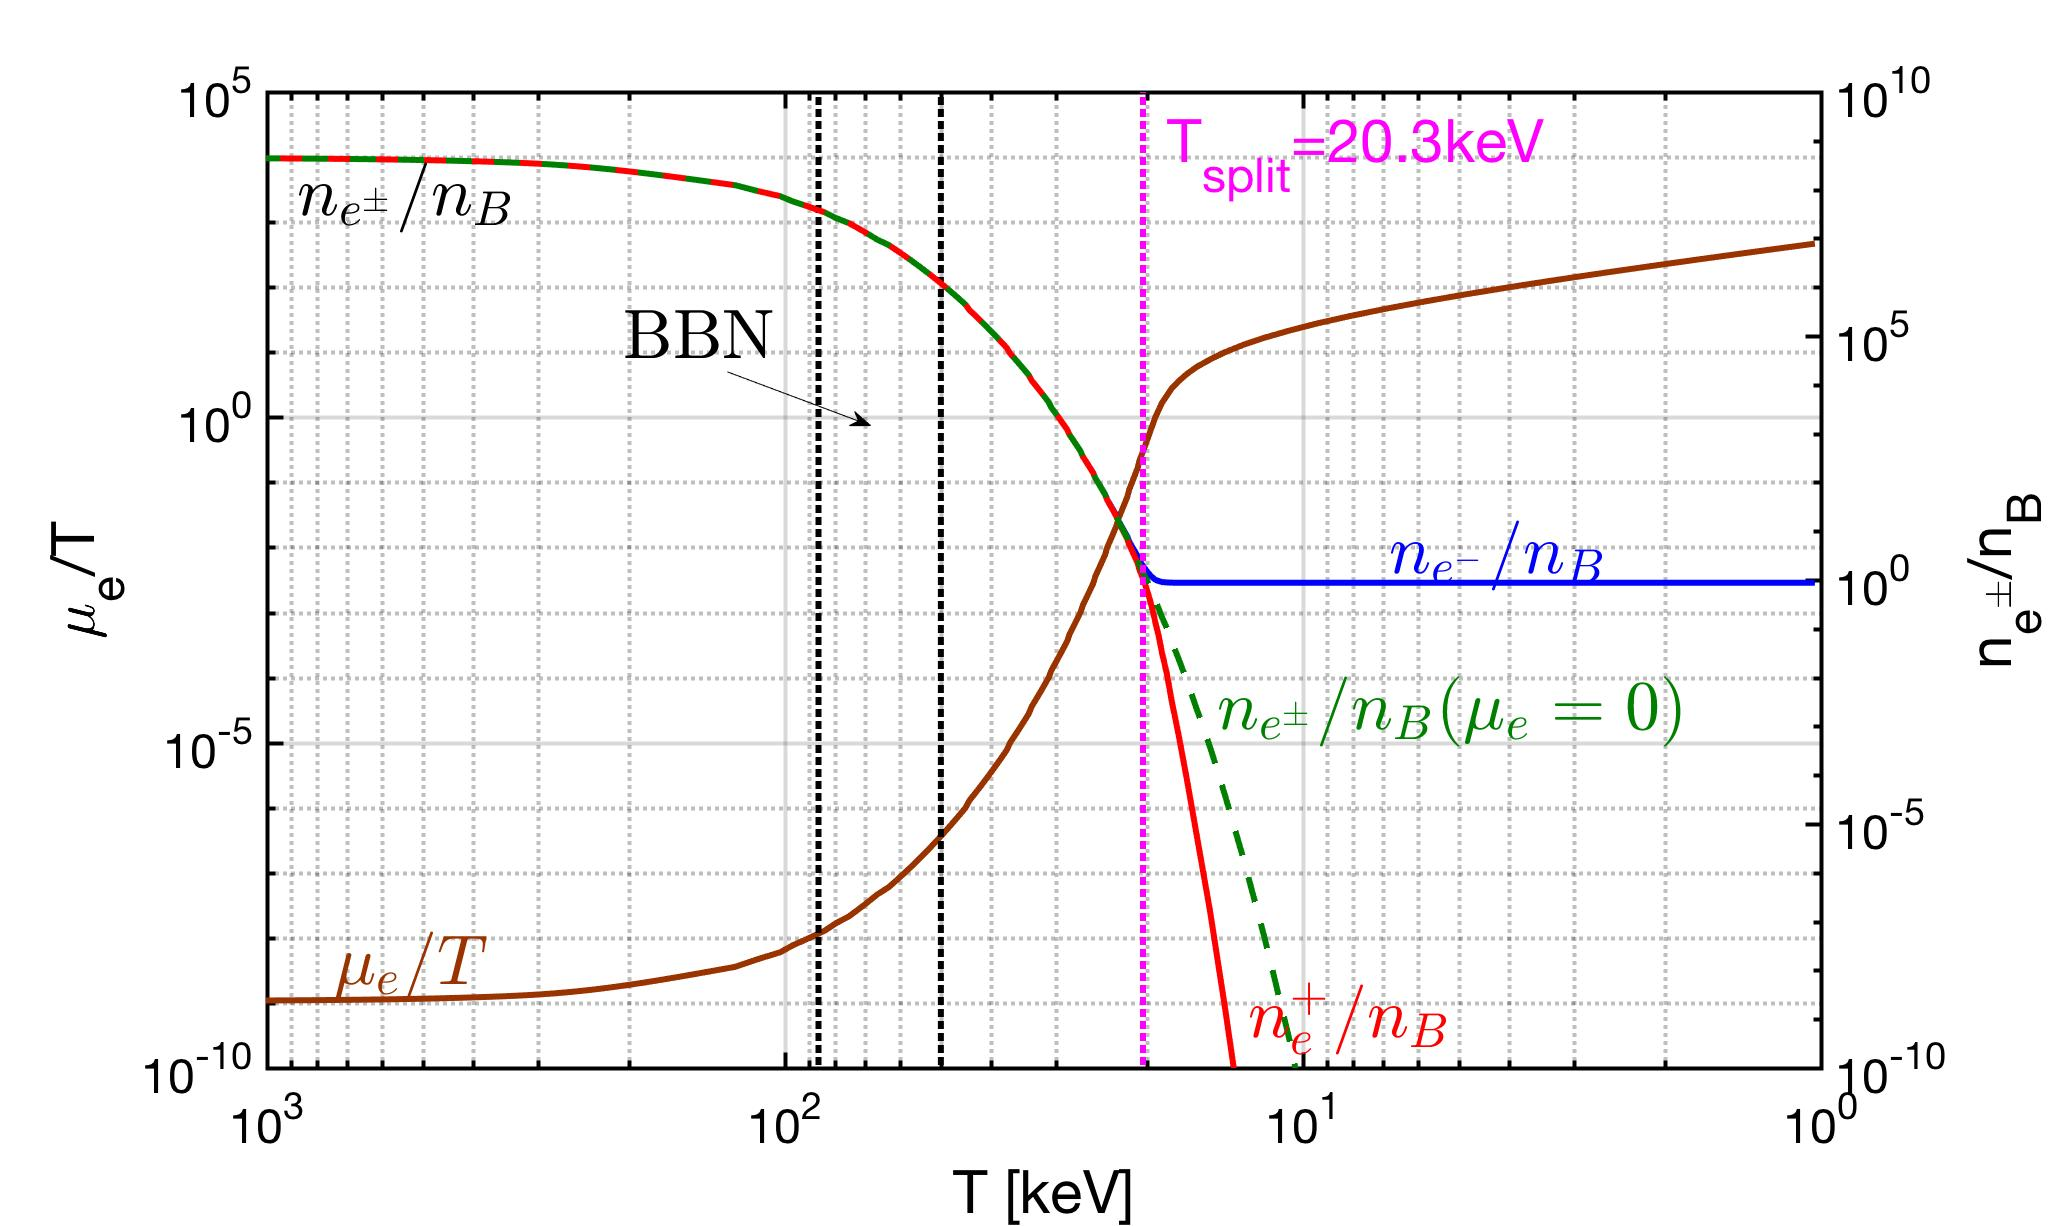
\includegraphics[width=0.90\linewidth]{plots/chap03BBN/May152023_EPDensity_Chemical}}
\caption{Left axis: The chemical potential of electrons as a function of temperature by numerically solving Eq. (\ref{charge_neutral_cond3}) with $n_p/n_B=0.878$ and $n_B/n_\gamma=6.05\times10^{-10}$. Right axis: the ratio of electron (positron) number density to baryon density as a function of temperature. The solid blue line is the electron density, the red dashed line is the positron density, and the green dotted line is the number density with $\mu_e=0$. When $T=20.3\,\mathrm{keV}$ (the purple vertical line) positron density decreases rapidly because of the annihilation. The vertical black dotted lines represent BBN temperature range $86\,\mathrm{keV}>\mathrm{T_{BBN}}>50\,\mathrm{keV}$}
\label{BBN:Electron}
\end{figure}
%%%%%%%%%%%%%%%%%%%%%%%%%%%%%%%%%

In Fig.~\ref{BBN:Electron} (left axis), we solve Eq.~(\ref{charge_neutral_cond3}) numerically and plot the electron chemical potential as a function of temperature with the following parameters: proton concentration $X_p=0.878$ from observation~\cite{ParticleDataGroup:2022pth} and $n_B/n_\gamma=6.05\times10^{-10}$ from CMB. We can see the value of chemical potential is comparatively small $\mu_e/T\approx10^{-6}\sim10^{-7}$ during the BBN temperature range, implying an equal number of electrons and positrons in plasma. The ratio of electron (positron) number density to baryon density shows that the Universe was filled with an electron-positron rich plasma during the accepted BBN temperature range. For example, when the temperature is around $T=70\,\mathrm{keV}$, the density of electrons and positrons is comparatively large $n_{e^\pm}\approx10^7\,n_B$. At $90$\,keV, the electron and positron density is near the solar core density, see Fig.~19 in Ref.~\cite{Rafelski:2023emw}. Later when the temperature is around $T=20.3\,\mathrm{keV}$, the positron density decreases, transforming the pair-plasma to an electron-baryon plasma.





%%%%%%%%%%%%%%%%%%%%%%%%%%%%%%%%%%%%%%%%%%%%%%%%%%%%%
%\subsubsection\label{sec:relax}
\paragraph{Electron-positron plasma damping rate:}
To find the damping rate in the BBN electron-positron plasma, we considered the major scatterings between photons and $e^+e^-$ pairs: inverse Compton scattering, M{\o}ller scattering, and Bhabha scattering
\begin{align}
&e^\pm+\gamma\longrightarrow e^\pm+\gamma,\qquad e^\pm+e^\pm\longrightarrow e^\pm+e^\pm,\qquad e^\pm+e^\mp\longrightarrow e^\pm+e^\mp\,.
\end{align}
% In general, to evaluate the reaction rate in two-body reaction $1+2\rightarrow3+4$ in the Boltzmann approximation we can use reaction cross-section $\sigma(s)$ and the relation from Ref.~\cite{Letessier:2002ony}:
% \begin{align}\label{GeneralRate}
% R_{12\rightarrow34}=\frac{g_1g_2}{32\pi^4}\frac{T}{1+I_{12}}\!\!\int^\infty_{s_{th}}\!\!\!\!ds\,\sigma(s)\frac{\lambda_2(s)}{\sqrt{s}}\!K_1\!\!\left({\sqrt{s}}/{T}\right),
% \end{align}
% where $K_1$ is the first-order Bessel function and the K\"{a}ll\'{e}n function $\lambda_2(s)$ is defined as
% \begin{align}
% \lambda_2(s)=\left[s-(m_1+m_2)^2\right]\left[s-(m_1-m_2)^2\right],
% \end{align}
% with $m_{1/2}$ and $g_{1/2}$ are the masses and degeneracies of initial interacting particles. The factor $1/(1+I_{12})$ is introduced to avoid double counting of indistinguishable pairs of particles, we have $I_{12}=1$ for identical particles and $I_{12}=0$ otherwise. 

% The two-body cross-section can be obtained by averaging the matrix element over the Mandelstam variable $t$. We have
% \begin{align}
% &\sigma_{e^\pm\gamma}=\frac{1}{16\pi(s-m_e^2)^2}\int^0_{-(s-m_e^2)^2/s}\!\!\!\!\!\!\!\!\!\!\!\!\!\!\!\!\! dt\, |M_{e^\pm\gamma}|^2,\\
% &\sigma_{e^-e^-}=\frac{1}{16\pi s(s-4m_e^2)}\int^0_{-(s-4m_e^2)}\!\!\!\!\!\!\!\!\!\!\!\!\!\!\!\!\!dt\, |M_{e^\pm e^\pm}|^2,\\
% &\sigma_{e^-e^+}=\frac{1}{16\pi s(s-4m_e^2)}\int^0_{-(s-4m_e^2)}\!\!\!\!\!\!\!\!\!\!\!\!\!\!\!\!\!dt\, |M_{e^\pm e^\mp}|^2.
% \end{align}
% The matrix element associated with inverse Compton scattering is given by~\cite{Kuznetsova:2009bq, Kuznetsova:2011wt}
% \begin{align}
% |M_{e^\pm\gamma}|^2\!&=32 \pi^2\alpha^2\bigg[4\left(\frac{m_e^2}{m_e^2-s}+\frac{m_e^2}{m_e^2-u}\right)^2\notag\\
% & -\frac{4m_e^2}{m_e^2-s}-\frac{4m_e^2}{m_e^2-u} -
% \frac{m_e^2-u}{m_e^2-s} -\frac{m_e^2-s}{m_e^2-u}\bigg],
% \end{align}
% and for M{\o}ller and Bhabha scattering we have respectively
% \begin{align}
% &|M_{e^{-}e^{-}}|^{2}\!=64\pi^{2}\alpha^{2}\bigg[
% \frac{s^{2}+u^{2}+8m_e^{2}(t-m_e^{2})}{2(t-m^2_{\gamma})^{2}} \notag\\ 
% &+\frac{{s^{2}+t^{2}}+8m_e^{2}
% (u-m_e^{2})}{2(u-m_{\gamma}^2)^{2}} + \frac{\left( {s}-2m_e^{2}\right)\left({s}-6m_e^{2}\right)}
% {(t-m_{\gamma}^2)(u-m_{\gamma}^2)} \bigg],
% \end{align}
% and
% \begin{align}
% &|M_{e^- e^+}|^{2}=64\pi^{2}\alpha^{2}
% \bigg[\frac{s^{2}+u^{2}+8m_e^{2}(t-m_e^{2})}{2(t-m^2_{\gamma})^{2}}\notag\\
% &+\frac{u^{2}+t^{2}+8m_e^{2}
% (s-m_e^{2})}{2(s-m^2_{\gamma})^{2}} + \frac{\left({u}-2m_e^{2}\right)\left({u}-6m_e^{2}\right)}
% {(t-m^2_{\gamma})(s-m^2_{\gamma})} \bigg],
% \label{M_fi_b}
% \end{align}
% where $s, t, u$ are the Mandelstam variables and we included the photon mass $m_\gamma$ to avoid singularity in reaction matrix elements. The photon mass in plasma is equal to the plasma frequency, in our case we have~\cite{Kislinger:1975uy}
% \begin{equation}
% m^2_\gamma=\omega^2_{p}=8\pi\alpha\int\frac{d^3p_e}{(2\pi)^3}\left(1-\frac{p_e^2}{3E_e^2}\right)\frac{f_- +f_+}{E_e},
% \end{equation}
% where $f_-$ and $f_+$ are the single-particle distribution functions for electrons and positrons respectively, and $E_e=\sqrt{p_e^2+m^2_e}$ is the electron energy. In the BBN temperature range $m_e\gg T$ and if we consider the non-relativistic electron and positron plasma
% \begin{align}
% m^2_\gamma=\frac{4\pi\alpha}{2m_e}\left(\frac{2m_eT}{\pi}\right)^{3/2}e^{-m_e/T}\cosh\left(\frac{\mu_e}{T}\right).
% \end{align}

% Substituting the cross-sections into Eq.~(\ref{GeneralRate}), the thermal reaction rate per volume for inverse Compton scattering can be written as
% \begin{align}
% R_{e^\pm\gamma}=\frac{g_eg_\gamma}{16\left(2\pi\right)^5}T\int_{m_e^2}^\infty\!\!\!\!ds\frac{K_1(\sqrt{s}/T)}{\sqrt{s}}\int^0_{-(s-m_e^2)^2/s}\!\!\!\!\!\!\!\!\!\!\!\!\!\!\!\!\!\!\!\!\!\!dt\, |M_{e^\pm\gamma}|^2,
% \end{align} 
% for M{\o}ller and Bhabha scattering we have
% \begin{align}
% &R_{e^\pm e^\pm}=\frac{g_eg_e}{16\left(2\pi\right)^5}T\!\!\int_{4m_e^2}^\infty\!\!\!\!ds\frac{K_1(\sqrt{s}/T)}{\sqrt{s}}\int^0_{-(s-4m_e^2)}\!\!\!\!\!\!\!\!\!\!\!\!\!\!\!\!\!\!\!\!\!\!dt\,|M_{e^\pm e^\pm}|^2,\\
% &R_{e^\pm e^\mp}=\frac{g_eg_e}{16\left(2\pi\right)^5}T\!\!\int_{4m_e^2}^\infty\!\!\!\!ds\frac{K_1(\sqrt{s}/T)}{\sqrt{s}}\int^0_{-(s-4m_e^2)}\!\!\!\!\!\!\!\!\!\!\!\!\!\!\!\!\!\!\!\!\!\!dt\,|M_{e^\pm e^\mp}|^2.
% \end{align}


%%%%%%%%%%%%%%%%%%%%%%%%%%%%%%%%%%%%%%%%%
\begin{figure}[h!]
\begin{center}
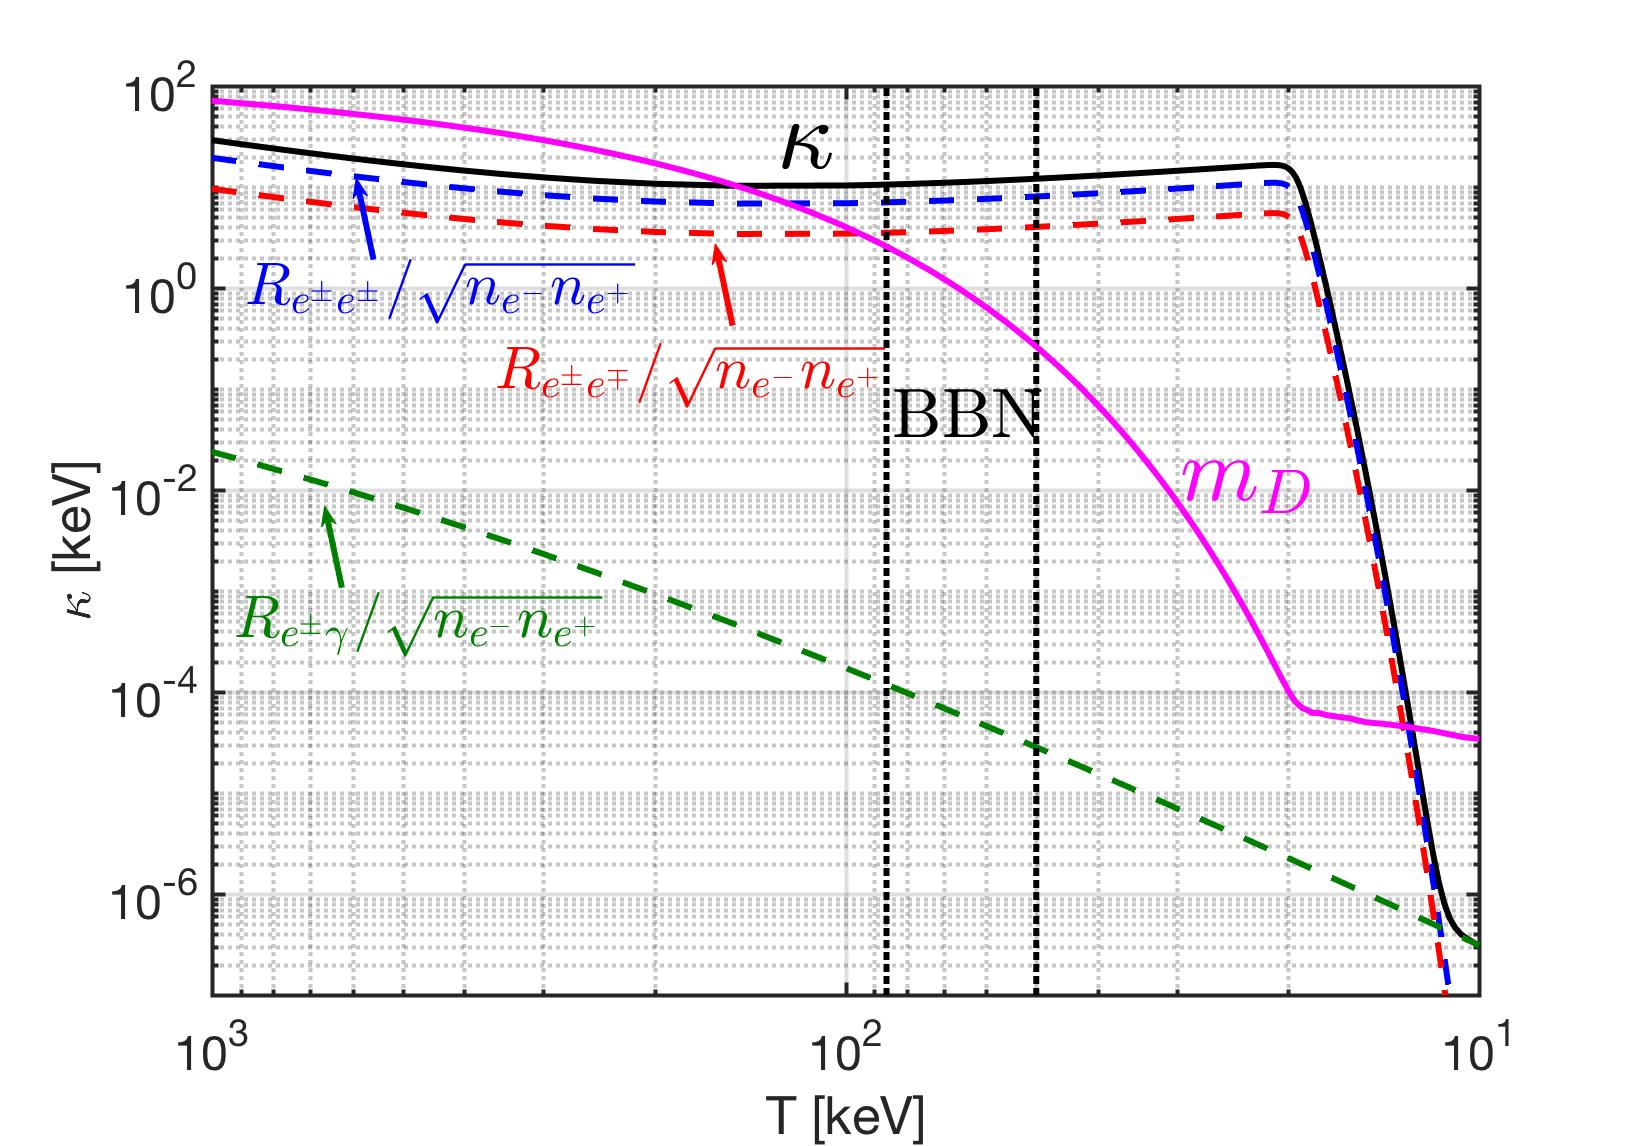
\includegraphics[width=0.95\linewidth]{plots/chap03BBN/May152023Kappa_EPPlasma002}
%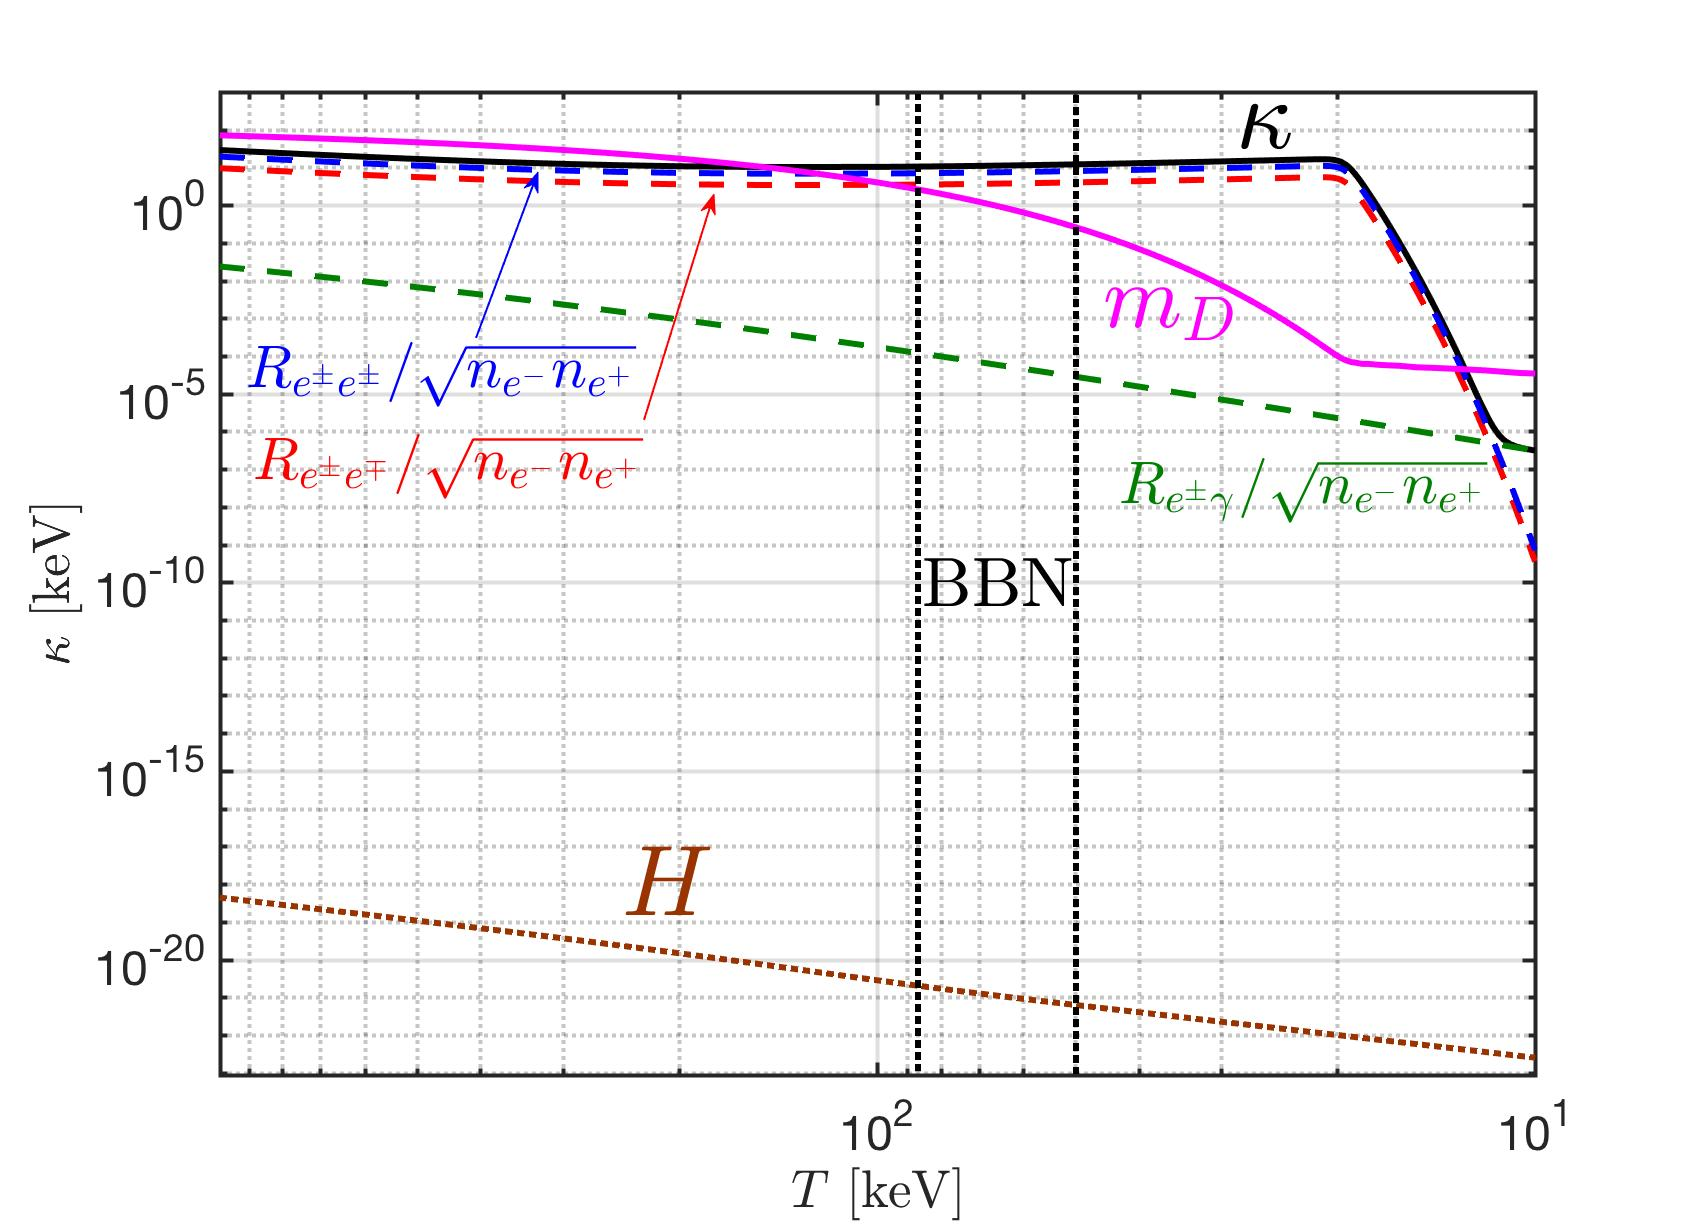
\includegraphics[width=0.95\linewidth]{May152023Kappa_EPPlasma}
\caption{\cccite{Grayson:2023flr}, adapted from Ref.~\cite{Grayson:2023flr} and thesis of C.T.Yang \cite{Yang:2024ret}. The relaxation rate $\kappa$ as a function of temperature in non-relativistic electron-positron plasma. We present reaction rates for M{\o}ller scattering $R_{e^\pm e^\pm}$ (blue dashed line), Bhabha scattering $R_{e^\pm e^\mp}$ (red dashed line), and inverse Compton scattering $R_{e^\pm \gamma}$ (green dashed line). The average relaxation rate from \req{Eq:Kappa}  is shown as a black solid line. The vertical black dotted lines represent BBN temperature range $86\,\mathrm{keV}>\mathrm{T_{BBN}}>50\,\mathrm{keV}$ during which the average relaxation rate is $\kappa=10\sim12$ keV. The dominant reactions during BBN are the M{\o}ller and Bhabha scatterings. The purple solid line represents the Debye mass given by Eq.~(\ref{eq:mL})}.
\label{Fig:RelaxationRate}
\end{center}
\end{figure}
%%%%%%%%%%%%%%%%%%%%%%%%%%%%%%%%%%%%%%%%%%%%%

C. T. Yang calculated these reaction rates by considering in-plasma tree-level QED scatterings using an infrared cutoff at $\omega_p$, which is the temperature-dependent effective photon mass in a plasma \cite{Yang:2024ret}.
In \rf{Fig:RelaxationRate}, we show the reaction rates $R$ for M{\o}ller, Bhabha, and inverse Compton scattering as a function of temperature. For temperatures $T>12.0$ keV, the dominant reactions in plasma are M{\o}ller and Bhabha scatterings between electrons and positrons. Thus, we can neglect the inverse Compton scattering in the BBN temperature range.
We then use these scattering rates in plasma to find the average damping rate:
\begin{align}\label{Eq:Kappa}
\kappa=\frac{R_{e^\pm e^\pm}+R_{e^\pm e^\mp}+R_{e^\pm\gamma}}{\sqrt{n_{e^-}n_{e^+}}}\approx\frac{R_{e^\pm e^\pm}+R_{e^\pm e^\mp}}{\sqrt{n_{e^-}n_{e^+}}},
\end{align}
where we neglect the inverse Compton scattering during BBN as discussed. The density function ${\sqrt{n_{e^-}n_{e^+}}}$ in the Boltzmann limit is given by
\begin{align}
{\sqrt{n_{e^-}n_{e^+}}}=\frac{g_e}{2\pi^3}T^3\left(\frac{m_e}{T}\right)^2K_2(m_e/T).
\end{align}
In \rf{Fig:RelaxationRate} that the total damping rate $\kappa$ given by  \req{Eq:Kappa}  is approximately constant $\kappa=10-12$ keV during the BBN. This value is much larger than the Debye mass defined below in Eq.~(\ref{eq:mL}). Below $T<20.3$ keV, the relaxation rate $\kappa$ decreases rapidly because the positrons disappear. At $T=12$\,keV, the inverse Compton scattering of remaining electrons becomes the dominant scattering process. 

%%%%%%%%%%%%%%%%%%%%%%%%%%%%%%%
\paragraph{Electron-positron plasma relaxation rate:}
In electron-positron plasma, the photon mass appears as $m_\gamma^2$ in the transition matrices for M{\o}ller and Bhabha reactions, which is one of important parameters in the calculation of the relaxation rate in $e^\pm$ plasma. When evaluating M{\o}ller and Bhabha scattering, we include the temperature-dependent mass of the photon obtained in plasma theory without damping. In general, the effective mass of the photon depends on the property of the plasma. Considering the linear response theory, the dispersion relation for the photon in nonrelativistic $e^\pm$ plasma is given by~\cite{Formanek:2021blc}
\begin{align}\label{dispersion_damping}
w^2=|k|^2+\frac{w}{w+i\kappa}w_{pl}^2,
\end{align}
where $w_{pl}$ is the plasma frequency and $\kappa$ is the average collision rate of $e^\pm$ plasma. The effective plasma frequency in damped plasma can be solved by considering the case $|k|^2=0$~\cite{Formanek:2021blc}
\begin{align}\label{plasmafrequency_damped}
w_{\pm}=-i\frac{\kappa}{2}\pm\sqrt{w^2_{pl}-\frac{\kappa^2}{4}}.
\end{align}
It shows that the plasma frequency in damped plasma $w_\pm$ is a function of $\kappa.$  In this case, the effective photon mass in damped plasma is also a function of the scattering rate. We have
\begin{align}\label{PhotonMass_self}
m_\gamma=w_\pm(w_{pl},\kappa)=m_\gamma(w_{pl},\kappa),
\end{align}
where the photon mass $m_\gamma=w_+$ for the underdamped plasma $w_{pl}>\kappa/2$, and $m_\gamma=w_-$ for overdamped plasma $w_{pl}<\kappa/2$. Eq.~(\ref{PhotonMass_self}) shows that computed damping strength $\kappa$ is the dominant scale for collisional plasma and it is also the main parameter determining the photon mass in plasma. 

Substituting the effective photon mass Eq.~(\ref{PhotonMass_self}) into the definition of the average relaxation rate Eq.~(\ref{Kappa}), we obtain the self-consistent equation for damping rate $\kappa$ as 
\begin{align}\label{RealaxtionSelf}
\kappa\,&\left[\frac{g_e}{2\pi^3}T^3\left(\frac{m_e}{T}\right)^2K_2(m_e/T)\right]\notag\\&=\frac{g_eg_e}{32\pi^4}T\!\!\int_{4m_e^2}^\infty\!\!\!\!ds\frac{s(s-4m^2_e)}{\sqrt{s}}K_1(\sqrt{s}/T)
\bigg[\sigma_{e^\pm e^\pm}(s,w_{pl},\kappa)+\sigma_{e^\pm e^\mp}(s,w_{pl},\kappa)\bigg],
\end{align}
where the cross sections depend on the parameter $w_{pl}$ and $\kappa$, and the variable $\kappa$ appears on both sides of the equation so we need solve the equation numerically to determine the $\kappa$ value that satisfies this condition.

Depending on the nature of the plasma (overdamped or underdamped plasma), we can establish the photon mass in collision plasma based on two distinct conditions as follows:
\begin{itemize}
\item Case 1. The plasma frequency is larger than the collision rate $w_{pl}>\kappa/2$, we have
\begin{align}
m_\gamma=w_+=-i\frac{\kappa}{2}+\sqrt{w^2_{pl}-\frac{\kappa^2}{4}}.
\end{align}
\item Case 2. The plasma frequency is smaller than the collision rate $w_{pl}<\kappa/2$, we have
\begin{align}\label{PhotonMassPlasma}
m_\gamma=w_-=-i\left(\frac{\kappa}{2}+\sqrt{\frac{\kappa^2}{4}-w^2_{pl}}\right).
\end{align}
\end{itemize}
In Fig.~\ref{RelaxationRate002_fig} it shows that during the BBN temperature range $50\leqslant T\leqslant 86$ keV, the plasma frequency is smaller than the collision rate $w_{pl}<\kappa/2$.  In this case, the effective photon mass in collision plasma during BBN epoch is given by Eq.(\ref{PhotonMassPlasma}).

%%%%%%%%%%%%%%%%%%%%%%%%%%%%%%%%%
\begin{figure}  
%\includegraphics[width=0.95\linewidth]{KappaRateToT_May082023}
\centerline{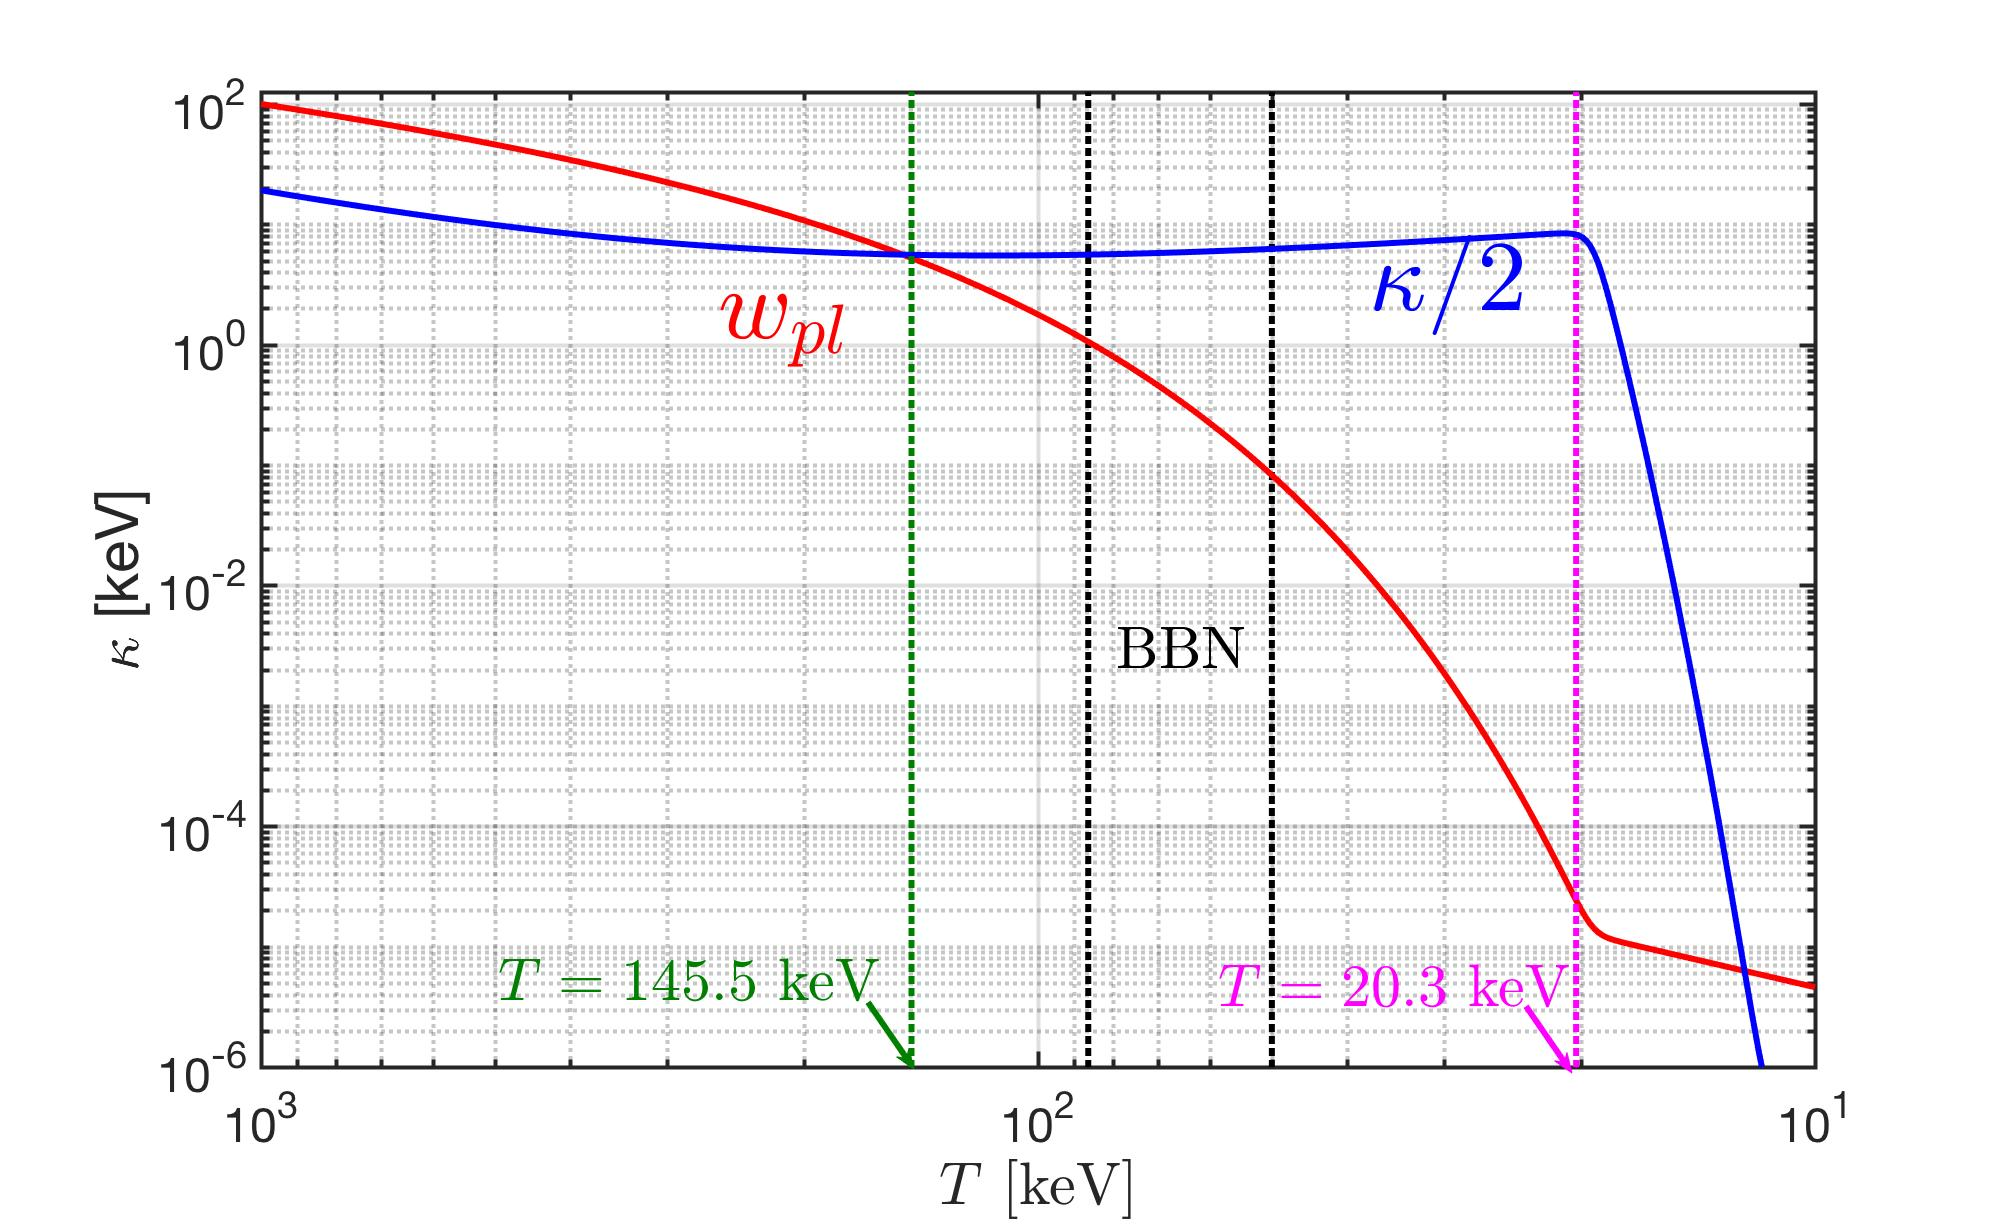
\includegraphics[width=\linewidth]{./plots/KappaElectronPhotonMass_Talk}}
\caption{The relaxation rate $\kappa/2$ (blue line) as a function of temperature in nonrelativistic electron-positron plasma. For comparison, we show the plasma frequency $\omega_{pl}$ in the red line. It shows that for $T>145.5$ MeV, the plasma frequency is larger than the collision rate $w_{pl}>\kappa/2$; for temperature $T<145.5$ MeV, we have $\kappa/2>w_{pl}$. For temperature $T<20.3$ keV, the composition of plasma is changed to electron and proton, which is beyond our current study because of unequal numbers of electrons and positrons}
\label{RelaxationRate002_fig} 
\end{figure}
%%%%%%%%%%%%%%%%%%%%%%%%%%%%%%%%%%%%%%%%%

To calculate the cross section for  M{\o}ller and Bhabha scattering we need to include the imaginary photon mass in the calculation of transition matrix elements. In general, the real part of photon mass in the calculation includes the effective photon-electron/positron scattering in plasma, and the imaginary part of photon mass contributes to the decay width of massive photon in plasma. To estimate the effect of photon mass on the damping rate $\kappa$, we first consider the effective mass corresponding to photon-electron/positron scattering in plasma, and leave the photon decay for future study.

For BBN temperature $50\leqslant T\leqslant 86$ keV,
we have $w_{pl}<\kappa$ and the effective photon mass can be approximated as
\begin{align}
m^2_\gamma=w_-w_-^\ast&=\left(\frac{\kappa}{2}+\sqrt{\frac{\kappa^2}{4}-w^2_{pl}}\right)^2
=\frac{\kappa^2}{2}\left[\left(1-\frac{2w^2_{pl}}{\kappa^2}\right)+\sqrt{1-\frac{4w^2_{pl}}{\kappa^2}}\right]\notag\\
&=\frac{\kappa^2}{2}\left[\left(1-\frac{2w^2_{pl}}{\kappa^2}\right)+\left(1-\frac{2w^2_{pl}}{\kappa^2}+\cdots\right)\right]\approx\kappa^2.
\label{PhotonMassPlasma002}
\end{align}
where we consider the limit $w^2_{pl}/\kappa^2\ll1$ and effective photon mass is equal to the average collision rate in plasma $m^2_\gamma\approx\kappa$.

Substituting the photon mass $m^2_\gamma=\kappa^2$ for overdamping plasma into the relaxation rate of electron-positron Eq.~(\ref{RealaxtionSelf}), and introducing the following dimensionless variables
\begin{align}
x=\sqrt{s}/T,\qquad a=m_\gamma/T=\kappa/T,\qquad b=m_e/T,
\end{align}

%%%%%%%%%%%%%%%%%%%%%%%%%%%%%%%%%%%%%%%%%%%%%%
\begin{figure} 
\centerline{
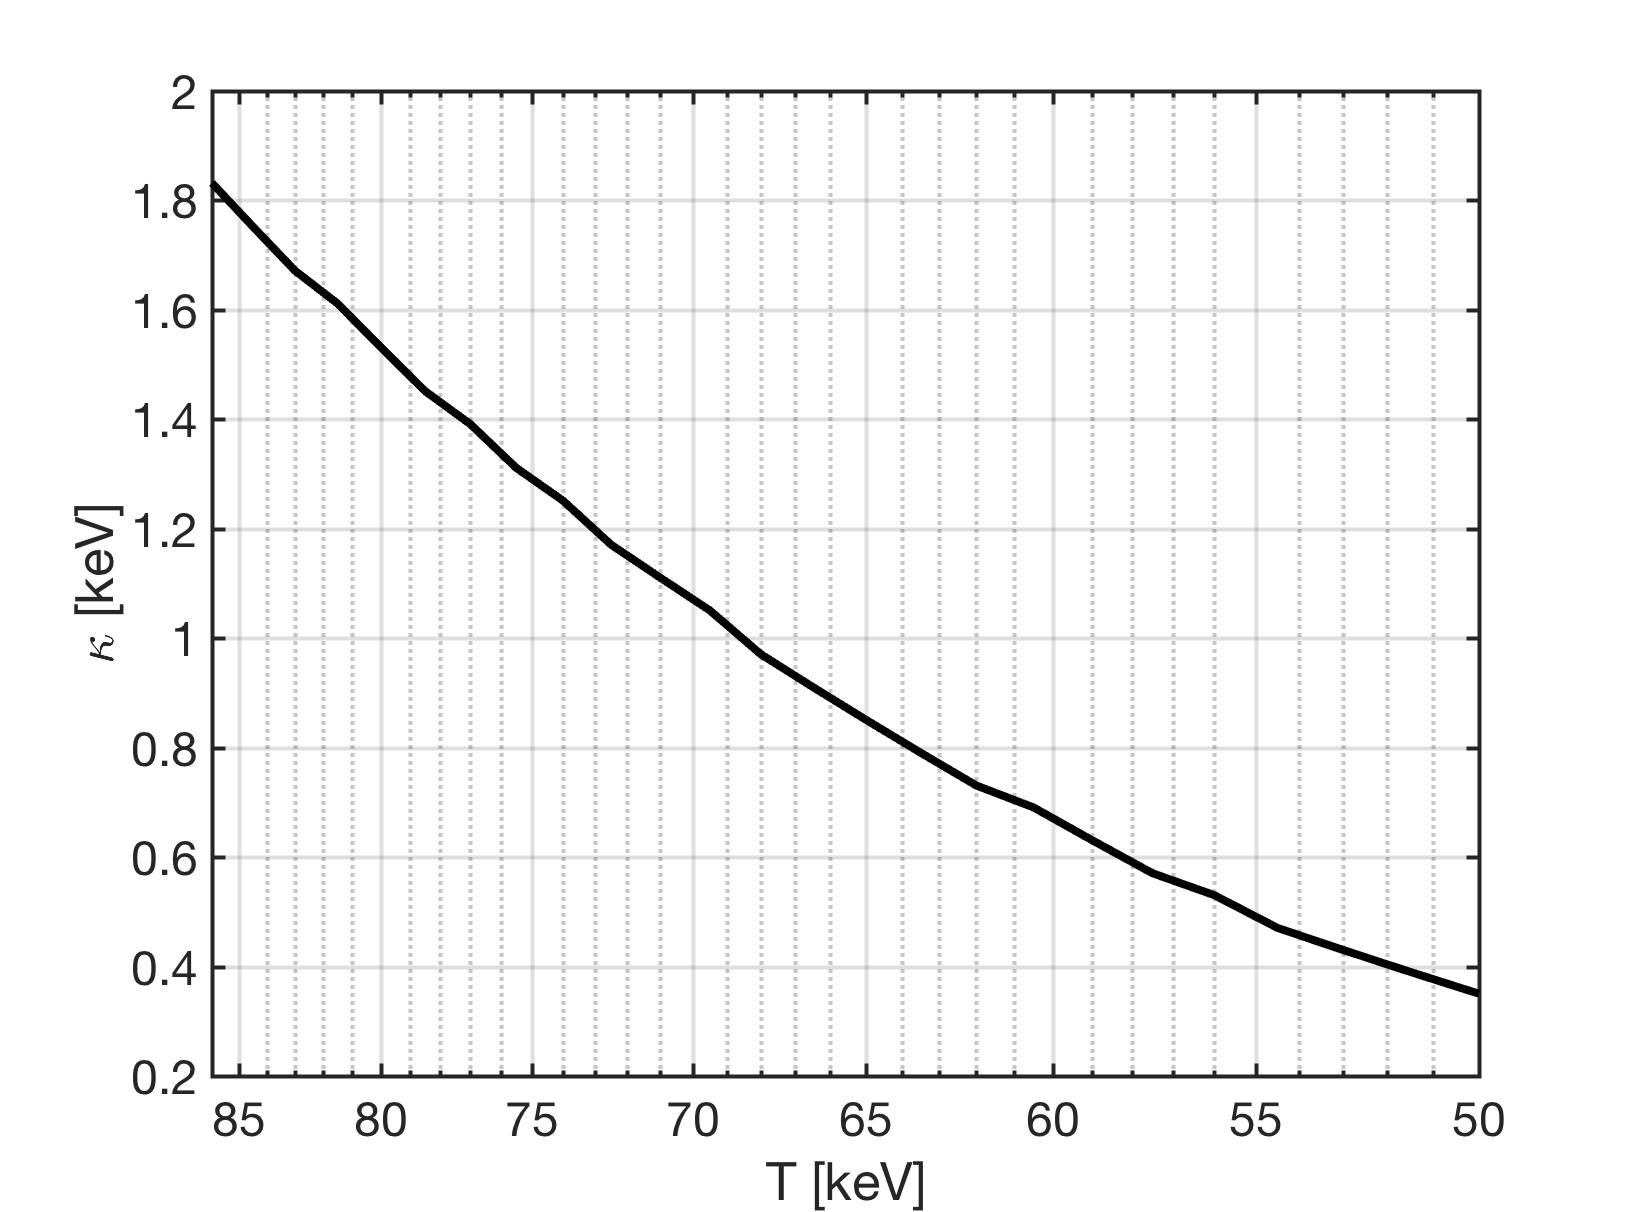
\includegraphics[width=\linewidth]{./plots/OverdampingKappa.jpg}}
\caption{The relaxation rate $\kappa$ that satisfies Eq.(\ref{Numerical_eq}) as a function of temperature $50\leqslant T\leqslant 86$\,keV. It shows that for overdamping plasma, we have $m^2_\gamma=\kappa^2$, and $\kappa=1.832$\,keV when $T=86$\,keV and $\kappa=0.350$\,keV when $T=50$\,keV. The minor fluctuations are a result of the restricted numerical precision}
\label{KappaSol.fig} 
\end{figure}
%%%%%%%%%%%%%%%%%%%%%%%%%%%%%%%%%%%%%%%%%%

then the relaxation rate of electron-positron can be written as
\begin{align}\label{Numerical_eq}
&\left[\frac{g_e}{2\pi^2}T^4\left(\frac{m_e}{T}\right)^{\!2}\!K_2(m_e/T)\right]\,\left(\frac{\kappa}{T}\right)\notag\\
&\qquad\qquad\qquad=\frac{g^2_e\alpha^2}{8\pi^3}T^4\!\!\int_{2b}^\infty\!dxK_1(x)\left[\mathcal{F}_{e^\pm e^\pm}(x,\kappa/T)+\mathcal{F}_{e^\pm e^\mp}(x,\kappa/T)\right],
\end{align}
where the functions $\mathcal{F}_{e^\pm e^\pm}$ and $\mathcal{F}_{e^\pm e^\mp}$ are given by
\begin{align}
\mathcal{F}_{e^\pm e^\pm}(x,a=\kappa/T)&=\left\{2\left[3a^2+4b^2+\frac{4(b^4-a^4)}{x^2-4b^2+2a^2}\right]\ln\left(\frac{a^2}{x^2-4b^2+a^2}\right)\right.\notag\\
&\left.+\frac{(x^2-4b^2)(8b^4+2a^4+3a^2x^2+2x^4-4b^2(2x^2+a^2))}{a^2(x^2-4b^2+a^2)}\right\}
\end{align}
and 
\begin{align}
\mathcal{F}_{e^\pm e^\mp}(x,a=\kappa/T)&=\left\{\frac{2x^2(a^2+x^2)-4b^4}{x^2-a^2}\ln\left(\frac{a^2}{x^2-4b^2+a^2}\right)\right.\notag\\
&+\frac{(x^2-4b^2)(3x^2+4b^2+2a^2)}{(x^2-a^2)}+\frac{x^6-12b^4x^2-16b^6}{3(x^2-a^2)^2}\notag\\
&\left.+\frac{(x^2-4b^2)(8b^4+2a^4+3a^2x^2+2x^4-4b^2(2x^2+a^2))}{a^2(x^2-4b^2+a^2)}\!\right\}.
\end{align}

To determine the $\kappa$ that satisfies Eq.~(\ref{Numerical_eq}), we can solve it numerically. 
In Fig.~\ref{KappaSol.fig}, we plot the relaxation rate $\kappa$ that satisfies Eq.~(\ref{Numerical_eq}) as a function of temperature $50\,\mathrm{keV} \leqslant T\leqslant 86$ keV. It shows that during the BBN temperature range, we have overdamping electron/positron plasma $w_{pl}<\kappa$, and the effective photon mass $m^2_\gamma=\kappa^2$. The relaxation rate $\kappa=1.832\sim0.350$ keV during the BBN temperature range, which is smaller than the relaxation rate without damping photon mass (See Fig.~\ref{RelaxationRate_fig}, where the relaxation rate $\kappa=10\sim12$ keV during the BBN temperature).

Our first estimation implies that the relaxation rate is sensitive to the photon mass in damped plasma. To address the self-consistent evaluation of damping  rate in plasma requires the development of a well-defined, self-consistent approach, where both damping and photon properties in plasma are determined in a mutually consistent manner. We aim to include the full photon mass effect (both real and imaginary parts) in the study and improve our calculation for the next step to complete the project.

